\section{Overall Architecture}
\begin{figure*}[t]
\centering
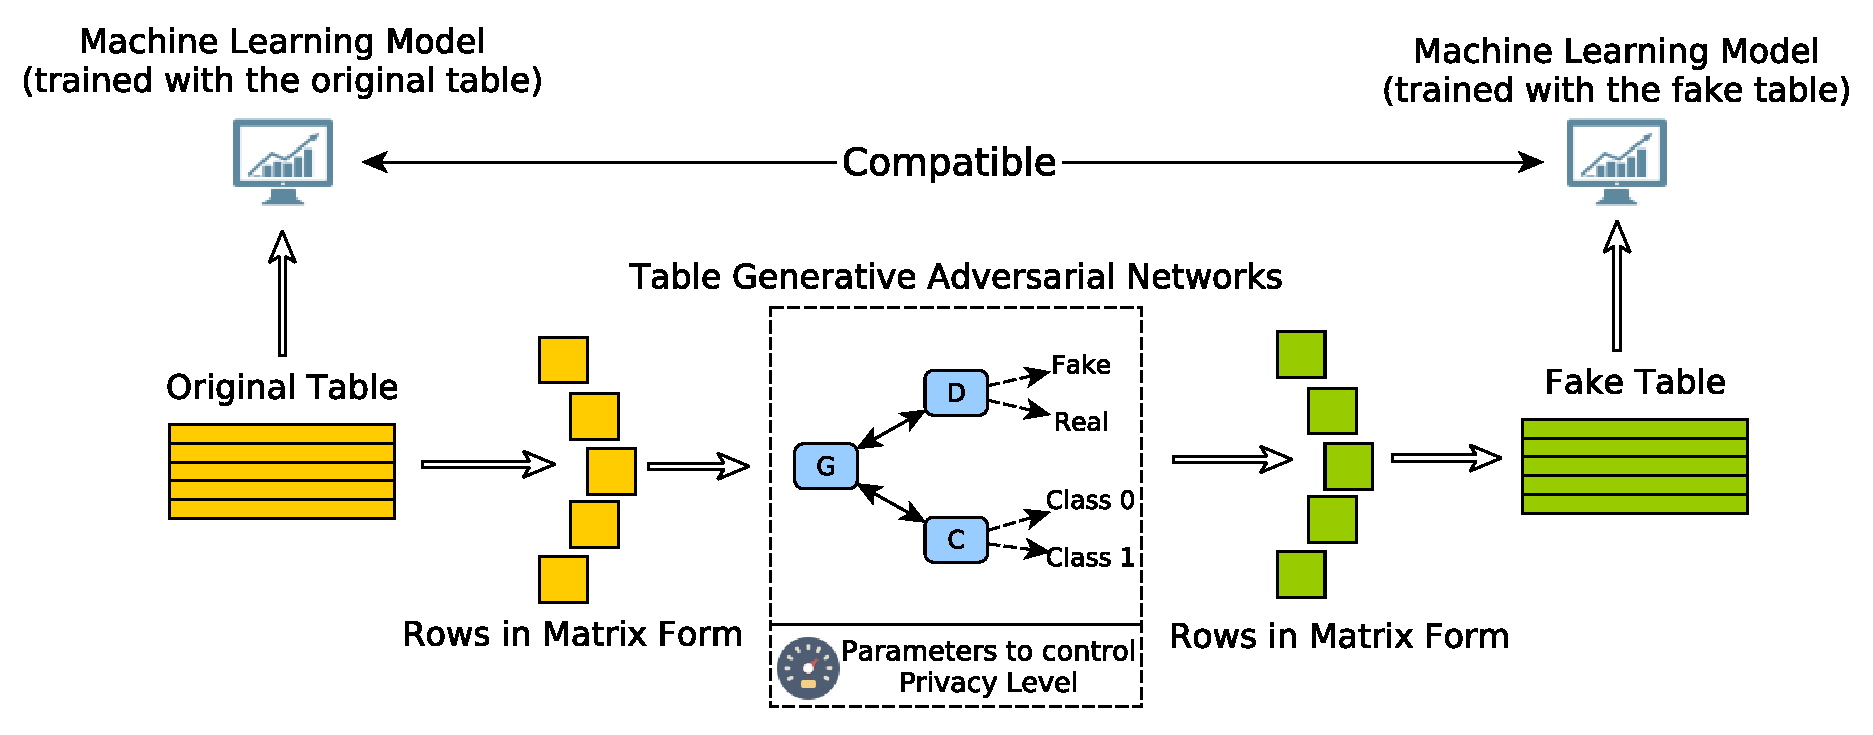
\includegraphics[width=0.8\textwidth]{tableGAN.eps}
\vspace{-1em}
\caption{The overall workflow of the proposed method. The fake table (marked in green) is generated by the proposed table-GAN trained using the original table (marked in yellow). Machine learning models trained using the fake table should show the same behaviors as models trained using the original table (i.e., model compatibility). Our goal is to achieve general model compatibility regardless of machine learning algorithms and tasks.}
\label{fig:tablegan}
\end{figure*}
% Existing data anonymization techniques remove identifying attributes of a table and transform quasi-identifiers (QIDs) using generalization \cite{samarati_2001_protecting}, micro-aggregation \cite{domingo_2005_ordinal,domingo_2002_practical}, etc.For example, Table~\ref{T:mot_origintable} shows an original table and Table~\ref{T:mot_anonymized} is its anonymized version using $k$-anonymity and $t$-closeness. In this example, ZIP code and age are QIDs, and salary and disease are sensitive attributes. As Table~\ref{T:mot_anonymized} shows, only QIDs are transformed and the sensitive attributes have their initial values.
% Existing data anonymization techniques remove identifying attributes of a table and transform quasi-identifiers (QIDs) using generalization \cite{samarati_2001_protecting}, micro-aggregation \cite{domingo_2005_ordinal,domingo_2002_practical}, etc. These techniques do not change values in sensitive attributes but only QIDs to satisfy a criteria requested by a privacy model such as $k$-anonymity or $t$-closeness. This means that the sensitive values are left intact in the anonymized table to maintain the usability in future analyses. For example, Table~\ref{T:mot_origintable} shows an original table and Table~\ref{T:mot_anonymized} is its anonymized version using $k$-anonymity and $t$-closeness. In this example, ZIP code and age are QIDs, and salary and disease are sensitive attributes. As Table~\ref{T:mot_anonymized} shows, only QIDs are transformed and the sensitive attributes have their initial values.

% Researchers in \cite{soria_2013_differential} and \cite{sun_2011_extended} have mentioned that while t-closeness can partially address the attribute disclosure problem, it can lead to noticeable utility losses in high dimensional data by breaking the link between the sensitive attributes and quasi-identifiers.
% , which is a main also applicable for $\epsilon$-differential privacy \cite{soria_2014_enhancing}.
% Other perturbation methods can change sensitive values. However, they are not proved for general model compatibility. In terms of model compatibility, anonymization is better than perturbation. See \cite{brickell_2008_cost} and \cite{domingo_2008_critique} for more detailed critiques about the shortcomings of current privacy models in the attribute disclosure problem.

% \textbf{We want to generate a synthetic table that does not contain any real information but its usability is maintained in future tasks such as classification and regression.} Recent achievements in generative models by the deep learning community enable this idea.

% \subsection{Problem Statement}
%  One more drawback of them is that a one-to-one relationship exists between the original table and the anonymized/perturbed table, and re-identification attacks are possible after discovering this relationship.
% Existing data anonymization/perturbation methods are not perfect because i) there is a chance of leaking sensitive information (i.e., attribute disclosure) and ii) a one-to-one relationship exists between the original table and the anonymized/perturbed table, and re-identification attacks are possible after discovering this relationship.

\begin{table}[t]
\small
\caption{Original Table. ZIP and Age are QIDs; Salary and Disease are sensitive attributes.}
\label{T:mot_origintable}
\vspace{-1em}
\begin{center}
\begin{tabular}{| c | c | c | c | c | }
\hline
No  & ZIP & Age & Salary & Disease \\
\hline
1 & 47677 &  29 & 3K &  AIDS  \\ 
2 & 47672 &  22 & 4K &  Ebola \\ 
3 & 47678 &  27 & 5K &  Cancer  \\ 
4 & 47905 &  53 & 6K &  AIDS  \\ 
5 & 47909 &  52 & 11K &  Ebola  \\  
6 & 47906 &  57 & 8K &  Heart Disease  \\  
% 7& 47605 &  30 & 7K &  Heart Disease  \\ 
% 8 & 47673 &  36 & 9K &  Ebola  \\  
% 9 & 47607 &  32 & 10K &  Cancer  \\ 
\hline
\end{tabular}
\end{center}
\caption{Table anonymized by 3-anonymity and 3-diversity. There are two equivalence classes and in each equivalence class, there are three records that are not distinguishable w.r.t. QIDs (i.e., 3-anonymity) and their sensitive values are all different (i.e., 3-diversity). \label{T:mot_anonymized}}
\vspace{-1em}
\begin{center}
\begin{tabular}{| c | c | c | c | c | }
\hline
No  & ZIP & Age & Salary & Disease \\
\hline
1 & 4767* &  $\leq$ 40 & 3K &  AIDS  \\ 
2 & 4767* &  $\leq$ 40 & 4K &  Ebola  \\ 
3 & 4767* &  $\leq$ 40 & 5k &  Cancer \\ \hline
4 & 4790* &  $\geq$ 50 & 6K &  AIDS  \\ 
5 & 4790* &  $\geq$ 50 & 11K &  Ebola  \\  
6 & 4790* &  $\geq$ 50 & 8K &  Heart Disease  \\ \hline
% 7& 4760* &  $\leq$ 40 & 4K &  Ebola  \\ 
% 8 & 4760* &  $\leq$ 40 & 7K &  Heart Disease   \\  
% 9 & 4760* &  $\leq$ 40 & 10K &  Cancer  \\  \hline
\end{tabular}
\end{center}
\end{table}

% \textbf{Our goal is to generate fake tables that show very good balance between them. In our fake table, there is no one-to-one correspondence. All identifiers, QIDs and sensitive attributes are fabricated by the proposed table-GAN}.

\subsection{Overall Workflow}
The overall workflow of our approach is presented in Figure~\ref{fig:tablegan}. It is processed in the following sequence:

\begin{itemize}
\item Records in the original table are converted into square matrix form; if needed, we pad with zeros. For example, a record that consists of 24 values can be converted into a $5 \times 5$ square matrix after padding a zero.
\item The proposed table-GAN is trained using the converted square matrices --- we will describe the details of the table-GAN in Section~\ref{sec:approach}.
\item The table-GAN generates many synthetic square matrices (i.e., synthetic records) that will be converted and merged into a table.
\item The generated fake table is shared with partners who will perform analyses and design machine learning models.
\item \textbf{The machine learning model trained using the synthetic table should be able to replace the model trained using the original table. In particular, we call this property \textit{model compatibility}.}
\end{itemize}

The generation process should have parameters to trade off between the level of privacy and the model compatibility. By decreasing the level of privacy, we can make records in the synthetic table similar to records in the original table and improve model compatibility.

\subsection{Data Types}
Our method is able to generate categorical, discrete and continuous values. Essentially, our model generates only continuous numerical values. For discrete values, however, we perform rounding at the final generation stage to convert continuous values into discrete values. For categorical values, the process is the same as for the discrete numerical values after label encoding (i.e., assigning an integer number to each category).%Editor: Please ensure that the intended meaning has been maintained in the above edit.

Table~\ref{T:example} presents an example that the proposed table-GAN is able to work with. SSN is a global identifier, gender and age are QIDs, cholesterol and diabetes are sensitive attributes, and in particular, diabetes contains ground-truth labels that can be used for model compatibility tests.

\begin{table}[t]
\small
\caption{An example table that can be synthesized by the proposed table-GAN\label{T:example}}
\vspace{-1em}
\begin{center}
\begin{tabular}{| c | c | c | c | c | }
\hline
SSN  & Gender & Age & Cholesterol & Diabetes \\
\hline
1 & Male &  29 & 65.5 &  0  \\ 
2 & Male &  22 & 130.9 &  1 \\ 
3 & Female &  27 & 190.1 &  1  \\ 
4 & Female &  43 & 78.4 &  0  \\
\hline
\end{tabular}
\end{center}
\end{table}

We leave other data types as future work. For instance, hierarchical recurrent neural networks are able to process a table that consists of string attributes~\cite{ElHihi:1995:HRN:2998828.2998898}. To our knowledge, there are no attempts to generate both of continuous numerical values and discrete strings within a single model.